\documentclass[11pt,letterpaper]{article}

\usepackage{times}
\usepackage{graphicx}
\usepackage{amsmath}
\usepackage{amssymb}
\usepackage{bm}
\usepackage{cite}
\usepackage{hyperref}
\usepackage{caption}
\usepackage{microtype}
\usepackage{booktabs}
\usepackage{geometry}
\usepackage{setspace}

\geometry{letterpaper, margin=1in}
\doublespacing
\emergencystretch=1.5em

\hypersetup{
    colorlinks=true,
    linkcolor=blue,
    citecolor=blue,
    urlcolor=blue
}

% Auto-generated by utils.metrics_logger. DO NOT EDIT DIRECTLY.
% Generated at: 2026-11-12T13:21:00.295025+00:00

\newcommand{\EngineBlenderVideoFrames}{72}
\newcommand{\EngineCampaignDesignCount}{4}
\newcommand{\EngineCfgBBallisticNetDeg}{7.5}
\newcommand{\EngineCfgBBarrierExitAj}{0.2508}
\newcommand{\EngineCfgBCodirDownPct}{66.7}
\newcommand{\EngineCfgBCodirUpPct}{73.3}
\newcommand{\EngineCfgBLoopResidualAj}{0.0974}
\newcommand{\EngineCfgBPanelsTotal}{3744}
\newcommand{\EngineCfgBPeakFzAttrPn}{-13.8213}
\newcommand{\EngineCfgBPeakFzRepPn}{2.7057}
\newcommand{\EngineCfgBPeakTauPosPnUm}{1.5491}
\newcommand{\EngineCfgBReleaseNetDeg}{323.8}
\newcommand{\EngineCfgBReleasePeakOmegaKrad}{50.52}
\newcommand{\EngineCfgBStrokeOneFzHighPn}{3.9264}
\newcommand{\EngineCfgBStrokeOneFzStdPn}{3.034}
\newcommand{\EngineCfgBStrokeOneTauHighPnUm}{1.0244}
\newcommand{\EngineCfgBStrokeOneTauRoomKPnUm}{0.5034}
\newcommand{\EngineCfgBStrokeOneTauScalarPnUm}{0.9126}
\newcommand{\EngineCfgBStrokeOneTauStdPnUm}{0.5031}
\newcommand{\EngineCfgBStrokeThreeFzHighPn}{-13.3968}
\newcommand{\EngineCfgBStrokeThreeFzStdPn}{-8.343}
\newcommand{\EngineCfgBStrokeThreeTauHighPnUm}{0.3627}
\newcommand{\EngineCfgBStrokeThreeTauRoomKPnUm}{0.1075}
\newcommand{\EngineCfgBStrokeThreeTauScalarPnUm}{0.2385}
\newcommand{\EngineCfgBStrokeThreeTauStdPnUm}{0.1073}
\newcommand{\EngineCfgBVibroNetDeg}{78.9}
\newcommand{\EngineCfgBWorkDownAj}{0.2337}
\newcommand{\EngineCfgBWorkPowerStrokesAj}{0.3482}
\newcommand{\EngineCfgBWorkUpAj}{0.1145}
\newcommand{\EngineCfgCBallisticNetDeg}{5.2}
\newcommand{\EngineCfgCBarrierExitAj}{0.3075}
\newcommand{\EngineCfgCCodirDownPct}{86.7}
\newcommand{\EngineCfgCCodirUpPct}{60}
\newcommand{\EngineCfgCLoopResidualAj}{0.0383}
\newcommand{\EngineCfgCPanelsTotal}{3744}
\newcommand{\EngineCfgCPeakFzAttrPn}{-15.0535}
\newcommand{\EngineCfgCPeakFzRepPn}{2.8786}
\newcommand{\EngineCfgCPeakTauPosPnUm}{0.7109}
\newcommand{\EngineCfgCReleaseNetDeg}{366.8}
\newcommand{\EngineCfgCReleasePeakOmegaKrad}{65.96}
\newcommand{\EngineCfgCStrokeOneFzHighPn}{4.0429}
\newcommand{\EngineCfgCStrokeOneFzStdPn}{3.152}
\newcommand{\EngineCfgCStrokeOneTauHighPnUm}{0.4849}
\newcommand{\EngineCfgCStrokeOneTauRoomKPnUm}{0.4674}
\newcommand{\EngineCfgCStrokeOneTauScalarPnUm}{0.9507}
\newcommand{\EngineCfgCStrokeOneTauStdPnUm}{0.4673}
\newcommand{\EngineCfgCStrokeThreeFzHighPn}{-10.9562}
\newcommand{\EngineCfgCStrokeThreeFzStdPn}{-7.5041}
\newcommand{\EngineCfgCStrokeThreeTauHighPnUm}{0.7061}
\newcommand{\EngineCfgCStrokeThreeTauRoomKPnUm}{0.4128}
\newcommand{\EngineCfgCStrokeThreeTauScalarPnUm}{0.6897}
\newcommand{\EngineCfgCStrokeThreeTauStdPnUm}{0.4124}
\newcommand{\EngineCfgCVibroNetDeg}{2}
\newcommand{\EngineCfgCWorkDownAj}{0.358}
\newcommand{\EngineCfgCWorkPowerStrokesAj}{0.3458}
\newcommand{\EngineCfgCWorkUpAj}{-0.0122}
\newcommand{\EngineCfgDBallisticNetDeg}{60.8}
\newcommand{\EngineCfgDBarrierExitAj}{0.2293}
\newcommand{\EngineCfgDCodirDownPct}{60}
\newcommand{\EngineCfgDCodirUpPct}{73.3}
\newcommand{\EngineCfgDLoopResidualAj}{0.0984}
\newcommand{\EngineCfgDPanelsTotal}{4440}
\newcommand{\EngineCfgDPeakFzAttrPn}{-11.9371}
\newcommand{\EngineCfgDPeakFzRepPn}{13.3255}
\newcommand{\EngineCfgDPeakTauPosPnUm}{1.5855}
\newcommand{\EngineCfgDReleaseNetDeg}{379.6}
\newcommand{\EngineCfgDReleasePeakOmegaKrad}{58.86}
\newcommand{\EngineCfgDStrokeOneFzHighPn}{9.5569}
\newcommand{\EngineCfgDStrokeOneFzStdPn}{6.3089}
\newcommand{\EngineCfgDStrokeOneTauHighPnUm}{1.1058}
\newcommand{\EngineCfgDStrokeOneTauRoomKPnUm}{0.5597}
\newcommand{\EngineCfgDStrokeOneTauScalarPnUm}{0.966}
\newcommand{\EngineCfgDStrokeOneTauStdPnUm}{0.5592}
\newcommand{\EngineCfgDStrokeThreeFzHighPn}{-12.4084}
\newcommand{\EngineCfgDStrokeThreeFzStdPn}{-7.7037}
\newcommand{\EngineCfgDStrokeThreeTauHighPnUm}{0.3455}
\newcommand{\EngineCfgDStrokeThreeTauRoomKPnUm}{0.0764}
\newcommand{\EngineCfgDStrokeThreeTauScalarPnUm}{0.2866}
\newcommand{\EngineCfgDStrokeThreeTauStdPnUm}{0.0763}
\newcommand{\EngineCfgDVibroNetDeg}{51}
\newcommand{\EngineCfgDWorkDownAj}{0.137}
\newcommand{\EngineCfgDWorkPowerStrokesAj}{0.3276}
\newcommand{\EngineCfgDWorkUpAj}{0.1907}
\newcommand{\EngineRMaxUm}{1.1}
\newcommand{\EngineRMinUm}{0.2}
\newcommand{\EngineSectorDeg}{90}
\newcommand{\EngineStrokeNm}{32}
\newcommand{\EngineSymCtrlBallisticNetDeg}{1.1}
\newcommand{\EngineSymCtrlBarrierExitAj}{0.0264}
\newcommand{\EngineSymCtrlCodirDownPct}{46.7}
\newcommand{\EngineSymCtrlCodirUpPct}{46.7}
\newcommand{\EngineSymCtrlLoopResidualAj}{0.0031}
\newcommand{\EngineSymCtrlPanelsTotal}{2352}
\newcommand{\EngineSymCtrlPeakFzAttrPn}{-3.164}
\newcommand{\EngineSymCtrlPeakFzRepPn}{1.6897}
\newcommand{\EngineSymCtrlPeakTauPosPnUm}{0.709}
\newcommand{\EngineSymCtrlReleaseNetDeg}{1.2}
\newcommand{\EngineSymCtrlReleasePeakOmegaKrad}{9.46}
\newcommand{\EngineSymCtrlStrokeOneFzHighPn}{1.6229}
\newcommand{\EngineSymCtrlStrokeOneFzStdPn}{1.3965}
\newcommand{\EngineSymCtrlStrokeOneTauHighPnUm}{-0.2274}
\newcommand{\EngineSymCtrlStrokeOneTauRoomKPnUm}{-0.3594}
\newcommand{\EngineSymCtrlStrokeOneTauScalarPnUm}{-0.3131}
\newcommand{\EngineSymCtrlStrokeOneTauStdPnUm}{-0.3593}
\newcommand{\EngineSymCtrlStrokeThreeFzHighPn}{-7.6201}
\newcommand{\EngineSymCtrlStrokeThreeFzStdPn}{-2.5162}
\newcommand{\EngineSymCtrlStrokeThreeTauHighPnUm}{-0.1847}
\newcommand{\EngineSymCtrlStrokeThreeTauRoomKPnUm}{0.01}
\newcommand{\EngineSymCtrlStrokeThreeTauScalarPnUm}{0.0072}
\newcommand{\EngineSymCtrlStrokeThreeTauStdPnUm}{0.01}
\newcommand{\EngineSymCtrlVibroNetDeg}{1.9}
\newcommand{\EngineSymCtrlWorkDownAj}{0.0078}
\newcommand{\EngineSymCtrlWorkPowerStrokesAj}{-0.0295}
\newcommand{\EngineSymCtrlWorkUpAj}{-0.0373}


\title{\textbf{The Fractal Casimir Engine: Co-Directional Dual-Stroke Torque, \texorpdfstring{$(z,\theta)$}{(z, theta)} Cycle Mapping, and Reciprocating-Rotary Rectification in Chiral Cantor NEMS}}

\author{\textbf{Goren Gordon} \\
Department of Informatics, Indiana University Bloomington \\
Bloomington, Indiana, USA \\
E-mail: \href{mailto:goren@gorengordon.com}{goren@gorengordon.com}}

\date{\today}

\begin{document}

\maketitle

\begin{abstract}
Interdigitated concentric Cantor-ring nanoelectromechanical systems (NEMS) in true vacuum ($\varepsilon_{\rm bg}=1.0$) switch their axial Casimir force sign between slot-aligned repulsion ($F_z > 0$) and recessed landing-pad attraction ($F_z < 0$), yet azimuthal reflection symmetry in conventional rotary quantum clutches yields vanishing torque ($\tau_\theta = 0$) at both equilibrium states. Here we introduce and map the \emph{Fractal Casimir Engine}: a family of chiral multi-scale Cantor NEMS architectures across $R \in [\EngineRMinUm{}, \EngineRMaxUm{}]\ \mu\text{m}$ with $\EngineSectorDeg{}^\circ$ cyclic sector periodicity and a $\EngineStrokeNm{}\text{ nm}$ vertical reciprocation stroke designed so that \emph{both} upward repulsive lift ($F_z > 0, \dot{z} > 0$) and downward landing-pad attraction ($F_z < 0, \dot{z} < 0$) simultaneously generate forward azimuthal torque ($\tau_\theta > 0$) in the same rotational direction. Using a regularized tangential surface-current 3D cyclic boundary-element (BEM) scattering formulation with exact co-rotating $(z,\theta)$ derivatives to evaluate the Casimir interaction energy $E_C(z,\theta)$, axial force $F_z = -\partial E_C/\partial z$, and azimuthal torque $\tau_\theta = -\partial E_C/\partial\theta$ in a single LU factorization pass per mode across $\EngineCampaignDesignCount{}$ structural families, we benchmark three chiral architectures against a reflection-symmetric $N=2$ Cantor control: (i) a Manhattan vertical-wall radial-taper and Vernier-staggered Cantor engine (\texttt{Config B}), (ii) a helically pitched Cantor louver turbine (\texttt{Config C}), and (iii) a dual-stator push-pull Cantor cage (\texttt{Config D}). All three chiral designs achieve co-directional positive torque across both the repulsive up-stroke (reaching $+\EngineCfgBStrokeOneTauStdPnUm{}\text{ pN}\cdot\mu\text{m}$ in \texttt{Config B}, $+\EngineCfgCStrokeOneTauStdPnUm{}\text{ pN}\cdot\mu\text{m}$ in \texttt{Config C}, and $+\EngineCfgDStrokeOneTauStdPnUm{}\text{ pN}\cdot\mu\text{m}$ in \texttt{Config D}) and the attractive down-stroke ($+\EngineCfgBStrokeThreeTauStdPnUm{}$, $+\EngineCfgCStrokeThreeTauStdPnUm{}$, and $+\EngineCfgDStrokeThreeTauStdPnUm{}\text{ pN}\cdot\mu\text{m}$, respectively), harvesting $+\EngineCfgDWorkPowerStrokesAj{}\text{ aJ}$ of combined two-stroke work in \texttt{Config D} while satisfying conservative closed-loop closure ($|\oint dW| = \EngineCfgDLoopResidualAj{}\text{ aJ}$) in static equilibrium. Finally, coupled 2-DOF rigid-body dynamics demonstrate ballistic $(z \to \theta)$ stroke conversion, bounded vertical-vibration rectification, and continuous multi-sector spin-up ($\Delta\theta = +\EngineCfgDReleaseNetDeg{}^\circ$, peak angular velocity $\EngineCfgDReleasePeakOmegaKrad{}\text{ krad/s}$) under zero-torque pad-exit permittivity gating.
\end{abstract}

\newpage

\section{Introduction}
\label{sec:intro}

Quantum electromagnetic vacuum fluctuations give rise to macroscopic Casimir forces that dominate sub-100-nanometer nanomechanical dynamics \cite{casimir1948,bordag2009,rodriguez2011}. Although mirror-symmetric bodies in true vacuum ($\varepsilon_{\rm bg}=1.0$) invariably attract \cite{kennethklich2006}, three-dimensional interdigitation of metallic teeth inside open aperture slots breaks reflection symmetry and creates transverse saddle-point fringing fields that yield axial Casimir repulsion ($F_z > 0$) in true vacuum \cite{levin2010}. Organizing concentric interdigitated slots and teeth into a prefractal Cantor radial hierarchy \cite{shajesh2017} preserves nanoscale sidewall gaps across a micron-scale annulus, enabling unpowered rotary switching between disengaged slot-aligned repulsion and engaged landing-pad attraction.

A natural foundational question follows: \emph{can a concentric Cantor-ring architecture be shaped so that upward motion in the repulsive regime and downward motion in the attractive regime both propel the rotor in the same azimuthal direction, forming a reciprocating-rotary Fractal Casimir Engine?} Designing and analyzing such a device requires simultaneously honoring two physical principles:
\begin{enumerate}
    \item \textbf{Chiral Dual-Tier Force--Torque Coupling}: In the repulsive slot zone, the upper stator slot collars must lift the rotor upward ($F_z > 0$) while pulling it forward ($\tau_\theta = -\partial E_C/\partial\theta > 0$) toward the landing-pad zone. Over the recessed landing pad, the lower stator structures must pull the elevated rotor back downward ($F_z < 0$) while continuing to accelerate it forward in the \emph{same} $+\theta$ sense ($\tau_\theta > 0$).
    \item \textbf{Thermodynamic Loop Closure vs.\ Non-Equilibrium / Parametric Rectification}: For time-independent dispersive Gold surfaces in thermal equilibrium, $E_C(z,\theta)$ is a single-valued periodic conservative potential ($E_C(z,\theta+\EngineSectorDeg{}^\circ) = E_C(z,\theta)$), enforcing $\oint_{\mathcal{C}}(F_z\,dz + \tau_\theta\,d\theta) = 0$. Consequently, the mechanical work harvested across the repulsive up-stroke and attractive down-stroke is balanced in static equilibrium by an energy reset cliff $\Delta E_{\rm exit}$ at the pad-to-slot exit. Converting this conservative chiral cam into a continuously accelerating autonomous engine therefore requires breaking detailed balance without applying external torque---for example via pad-exit optical/phase-change permittivity gating, out-of-equilibrium thermal gradients \cite{antizza2008}, or purely vertical parametric base vibration.
\end{enumerate}

Here we formulate, verify, and dynamically simulate three chiral Cantor $N=2$ NEMS engine architectures alongside a matched symmetric control, coupling regularized 3D cyclic boundary-element $(E_C, F_z, \tau_\theta)$ mapping with 2-DOF rigid-body dynamics and 3D Blender trajectory visualization.

\section{Chiral Multi-Scale Cantor Engine Architectures}
\label{sec:architectures}

\begin{figure*}[t]
\centering
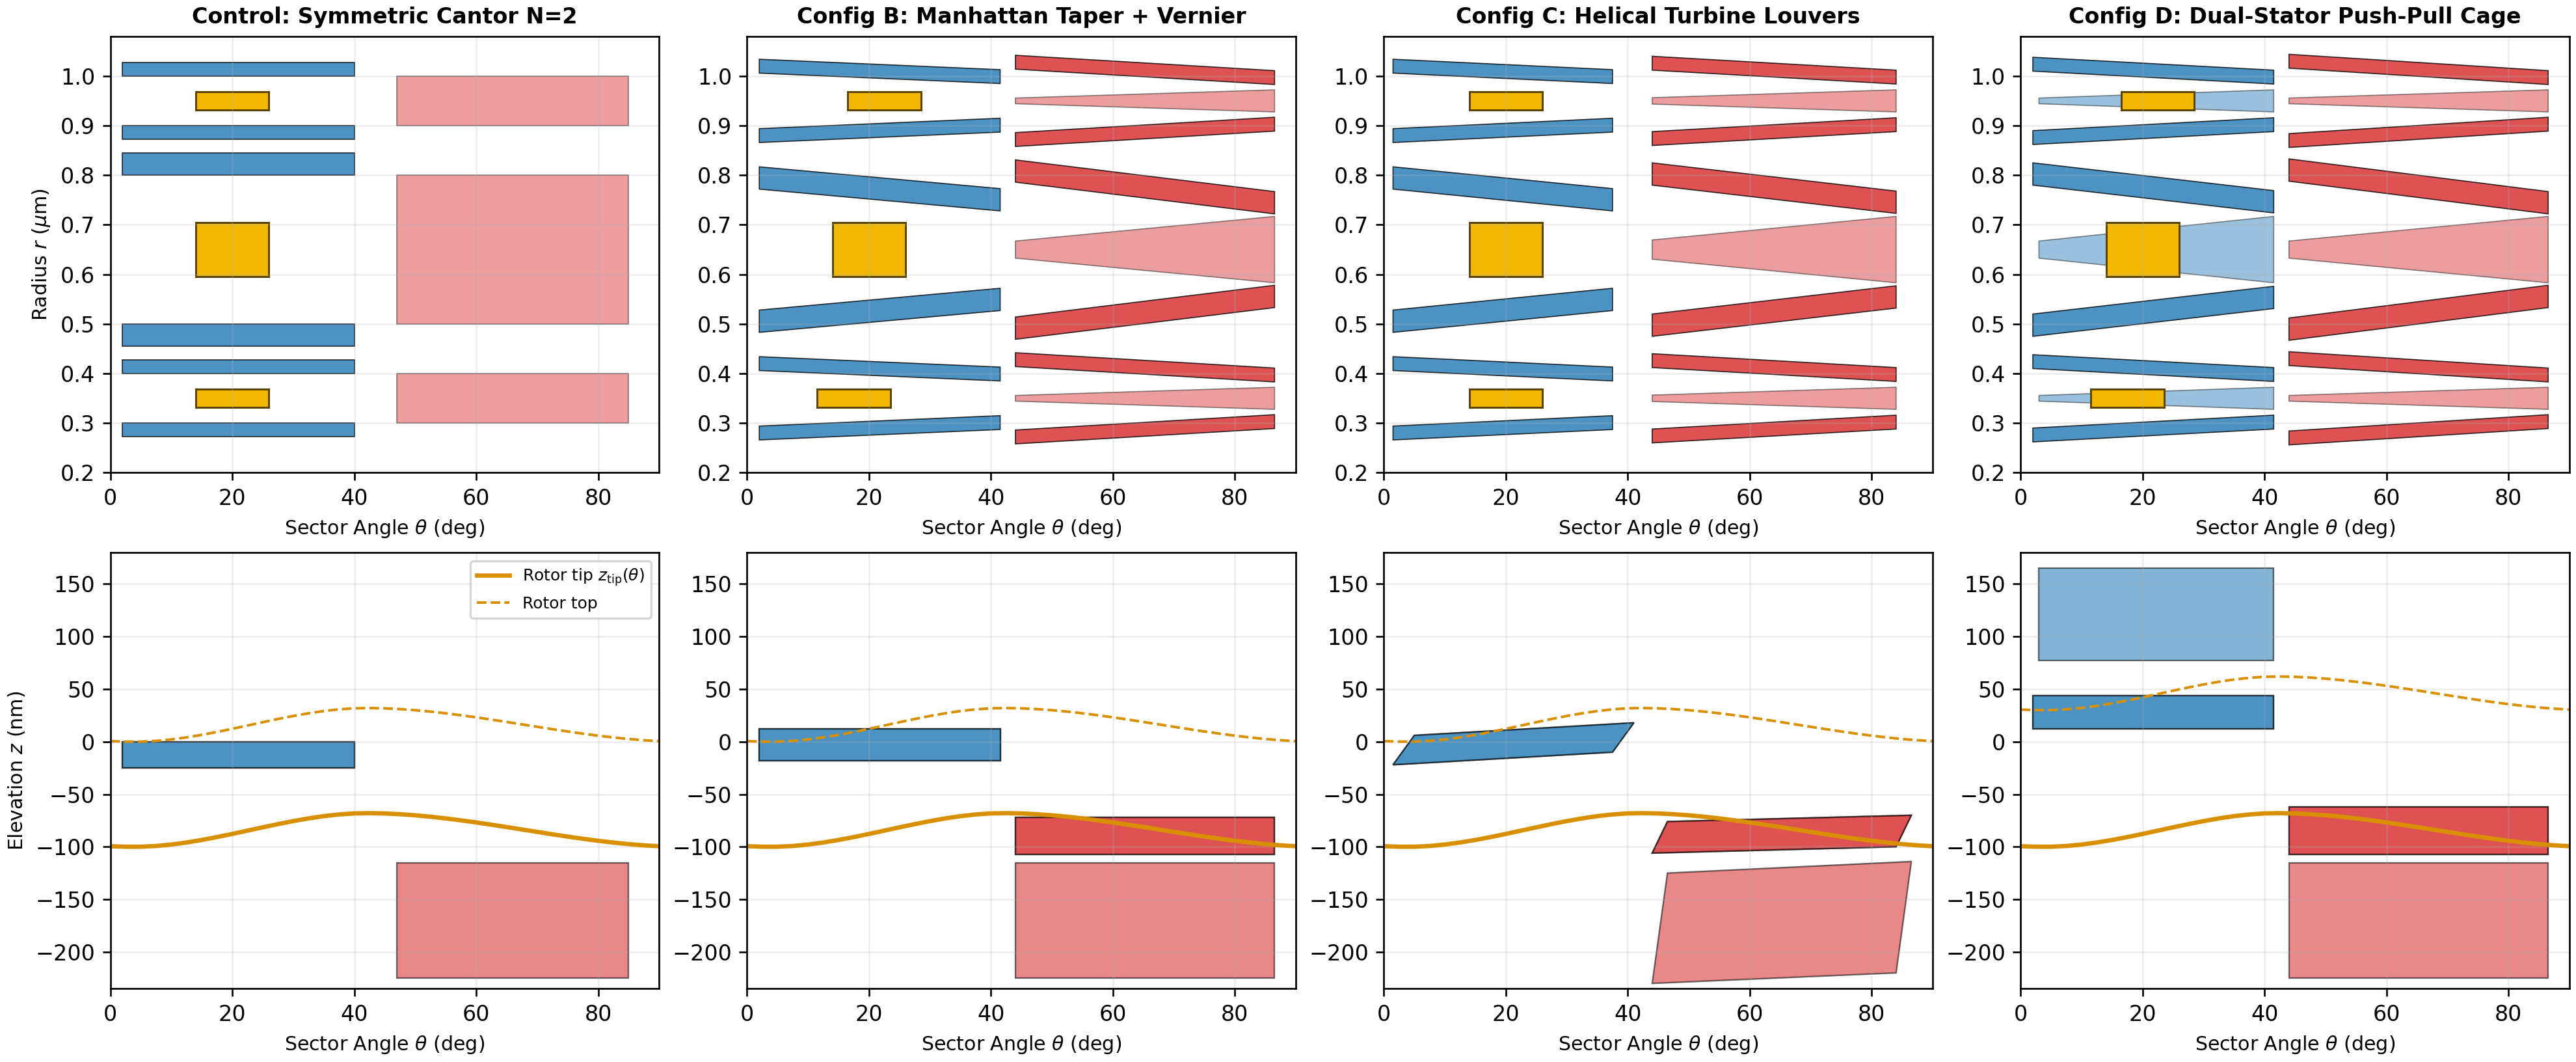
\includegraphics[width=0.98\textwidth]{figures/fig1_engine_architectures.png}
\caption{Planform $(r,\theta)$ and unfolded cylindrical $(\theta,z)$ cross-sections across the four evaluated $N=2$ Cantor architectures over $R \in [\EngineRMinUm{}, \EngineRMaxUm{}]\ \mu\text{m}$ ($\EngineSectorDeg{}^\circ$ sector period): reflection-symmetric control (\texttt{Sym\_Baseline\_CantorN2}), Manhattan radial-taper plus Vernier-staggered engine (\texttt{Config B}), helical louver turbine (\texttt{Config C}), and dual-stator push-pull cage (\texttt{Config D}).}
\label{fig:architectures}
\end{figure*}

All four architectures share an exact rational middle-third $N=2$ Cantor radial subdivision across $R \in [\EngineRMinUm{}, \EngineRMaxUm{}]\ \mu\text{m}$ with four-fold cyclic symmetry ($C_4$, $\EngineSectorDeg{}^\circ$ period) in true vacuum ($\varepsilon_{\rm bg}=1.0$, Fig.~\ref{fig:architectures}):
\begin{itemize}
    \item \textbf{Symmetric Cantor Control (\texttt{Sym\_Baseline\_CantorN2}, $\EngineSymCtrlPanelsTotal{}$ panels)}: Constant-gap upper repulsive slot collars and flat horizontal recessed landing pads symmetric about $\theta = 21^\circ$ and $\theta = 66^\circ$, respectively.
    \item \textbf{\texttt{Config B} --- Manhattan Radial-Taper \& Vernier Stagger ($\EngineCfgBPanelsTotal{}$ panels)}: Fabricable purely with vertical electron-beam lithography (EBL) walls. In Stroke~I, upper stator slot collars taper radially inward along $+\theta$, simultaneously increasing upward repulsive lift ($F_z > 0$) and pulling the rising tooth forward ($\tau_\theta > 0$). In Stroke~III, recessed horn-shaped landing pads expand radially along $+\theta$ while disjoint lower cheek rails below the tooth midplane narrow along $+\theta$, generating downward pull ($F_z < 0$) and co-directional forward torque ($\tau_\theta > 0$), smoothed by generation-indexed Vernier phase offsets.
    \item \textbf{\texttt{Config C} --- Helical Turbine Louvers ($\EngineCfgCPanelsTotal{}$ panels)}: Twists the Cantor rotor blades helically from bottom to top while pitching both the upper repulsive slot louvers and lower attractive louver pads in $(\theta,z)$.
    \item \textbf{\texttt{Config D} --- Dual-Stator Push-Pull Cage ($\EngineCfgDPanelsTotal{}$ panels)}: Pairs an upper attractive ceiling horn pad and high lifting slot collar in the up-stroke zone with a lower overhang-push collar and floor horn pad in the down-stroke zone around taller Cantor rotor teeth, doubling active stroke work across the $\EngineStrokeNm{}\text{ nm}$ vertical reciprocation window.
\end{itemize}

\section{Co-Rotating 3D Cyclic BEM Formulation for \texorpdfstring{$(E_C, F_z, \tau_\theta)$}{(EC, Fz, tau)}}
\label{sec:methods}

Along the Wick-rotated imaginary wavenumber axis $\kappa = \xi / c$, we evaluate the Casimir interaction energy $E_C$, axial force $F_z$, and azimuthal torque $\tau_\theta$ within the regularized tangential surface-current dyadic BEM (cross-checked against scalar Yukawa BEM) via four-sector cyclic Bloch decomposition ($m \in \{0,1,2,3\}$) summed over transverse magnetic and electric polarization channels ($\mathrm{ch}\in\{\mathrm{TM},\mathrm{TE}\}$):
\begin{equation}
E_C = \frac{\hbar c}{2\pi}\int_0^\infty d\kappa \sum_{m=0}^3 \sum_{\mathrm{ch}\in\{\mathrm{TM},\mathrm{TE}\}} \ln\det\mathbf{Y}_{m,\mathrm{ch}}(\kappa),
\quad
F_z = -\frac{\partial E_C}{\partial z},
\quad
\tau_\theta = -\frac{\partial E_C}{\partial \theta},
\end{equation}
where $\mathbf{Y}_{m,\mathrm{ch}} = \mathbf{I} - w_{\mathrm{ch}}^2 \mathbf{M}_{rr,m}^{-1}\mathbf{G}_{rs,m}\mathbf{M}_{ss,m}^{-1}\mathbf{G}_{rs,m}^\dagger$ weights dispersive Raki\'c Drude--Lorentz Gold evanescent Fresnel channels at $k_\parallel = k_{\rm eff}$ in true vacuum ($\varepsilon_{\rm bg}=1.0$). While the underlying single-layer tangential kernel is a regularized collocation model, $(F_z, \tau_\theta)$ are exact analytic derivatives of the discrete functional $E_C(z,\theta)$. Because $\det\mathbf{Y}_{m,\mathrm{ch}}$ is invariant under local $O(2)$ rotations of panel tangent frames, differentiating in the co-rotating rotor frame ($\partial_\theta \mathbf{q}_t = \hat{\mathbf{z}}\times\mathbf{q}_t$, $\partial_\theta \mathbf{t}_{t,\alpha} = \hat{\mathbf{z}}\times\mathbf{t}_{t,\alpha}$) renders both self-blocks strictly invariant ($\partial_\theta \mathbf{M}_{rr,m} = \mathbf{0}$, $\partial_\theta \mathbf{M}_{ss,m} = \mathbf{0}$), enabling pre-factorization of $\mathbf{M}_{rr,m}$ and $\mathbf{M}_{ss,m}$ and simultaneous extraction of $(E_C, F_z, \tau_\theta)$ in one linear solve per mode.

\section{2D \texorpdfstring{$(z,\theta)$}{(z, theta)} Cycle Landscapes, Multi-Solver Benchmarks, and Coupled Dynamics}
\label{sec:results}

\begin{figure*}[t]
\centering
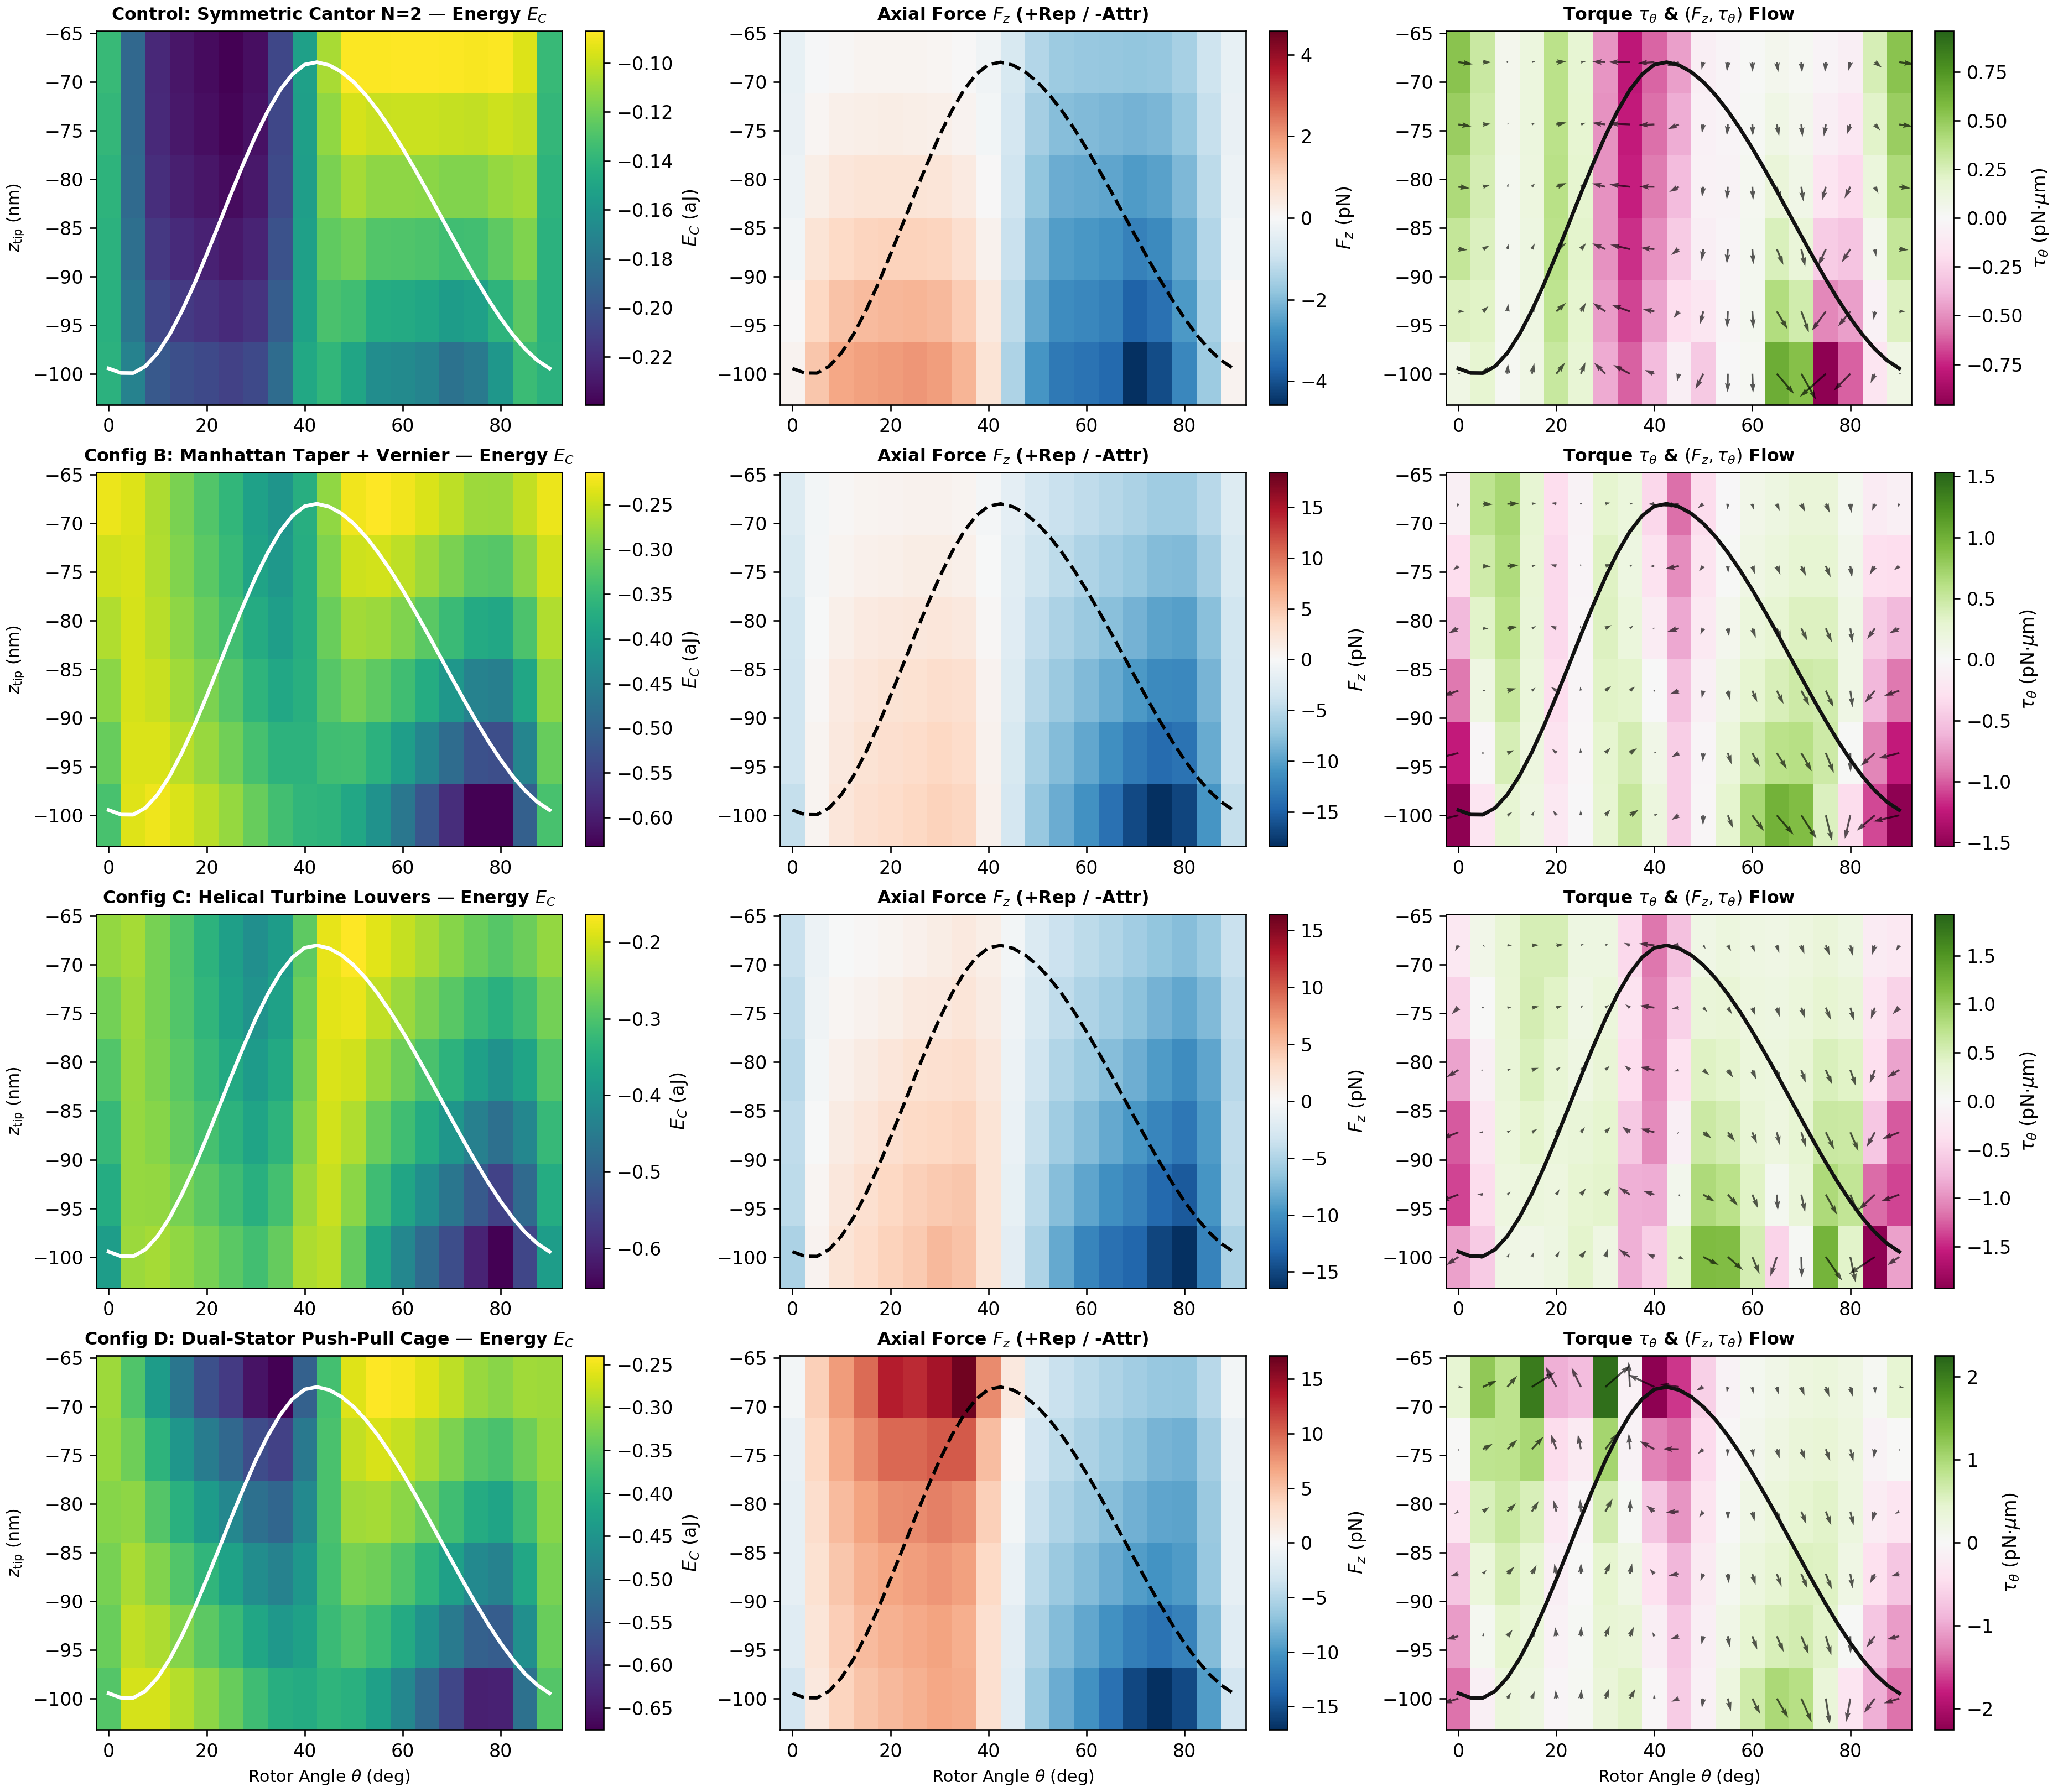
\includegraphics[width=0.98\textwidth]{figures/fig2_engine_2d_landscapes.png}
\caption{Complete 2D $(z_{\rm tip}, \theta)$ 3D Vector-Dyadic BEM landscapes of Casimir energy $E_C$, axial force $F_z$, and azimuthal torque $\tau_\theta$ with $(F_z,\tau_\theta)$ phase-space flow vectors and closed reciprocating cycle paths.}
\label{fig:landscapes}
\end{figure*}

\begin{table*}[t]
\centering
\caption{3D BEM force, torque, cycle energetics, and 2-DOF dynamical spin-up across the $\EngineCampaignDesignCount{}$ Cantor architectures in true vacuum ($\varepsilon_{\rm bg}=1.0$). Stroke~I is benchmarked at $(z_{\rm tip}=-92\text{ nm},\,\theta=22^\circ)$ and Stroke~III at $(z_{\rm tip}=-84\text{ nm},\,\theta=64^\circ)$ using baseline mesh $(n_r,n_{\phi,\rm tooth},n_{\phi,\rm arc},n_z,n_\xi)=(1,3,9,2,12)$ (`Std') and refined mesh $(2,4,12,2,16)$ (`Fine').}
\label{tab:engine_benchmarks}
\resizebox{\textwidth}{!}{%
\begin{tabular}{lcccc}
\toprule
Metric & \texttt{Sym Ctrl} & \texttt{Config B} & \texttt{Config C} & \texttt{Config D} \\
\midrule
Total 4-sector BEM panels (`Std') & $\EngineSymCtrlPanelsTotal{}$ & $\EngineCfgBPanelsTotal{}$ & $\EngineCfgCPanelsTotal{}$ & $\EngineCfgDPanelsTotal{}$ \\
Stroke I $F_z$ (Std / Fine BEM, pN) & $\EngineSymCtrlStrokeOneFzStdPn{}$ / $\EngineSymCtrlStrokeOneFzHighPn{}$ & $+\EngineCfgBStrokeOneFzStdPn{}$ / $+\EngineCfgBStrokeOneFzHighPn{}$ & $+\EngineCfgCStrokeOneFzStdPn{}$ / $+\EngineCfgCStrokeOneFzHighPn{}$ & $+\EngineCfgDStrokeOneFzStdPn{}$ / $+\EngineCfgDStrokeOneFzHighPn{}$ \\
Stroke I $\tau_\theta$ (Std / Fine, $\text{pN}\cdot\mu\text{m}$) & $\EngineSymCtrlStrokeOneTauStdPnUm{}$ / $\EngineSymCtrlStrokeOneTauHighPnUm{}$ & $+\EngineCfgBStrokeOneTauStdPnUm{}$ / $+\EngineCfgBStrokeOneTauHighPnUm{}$ & $+\EngineCfgCStrokeOneTauStdPnUm{}$ / $+\EngineCfgCStrokeOneTauHighPnUm{}$ & $+\EngineCfgDStrokeOneTauStdPnUm{}$ / $+\EngineCfgDStrokeOneTauHighPnUm{}$ \\
Stroke I $\tau_\theta$ (Scalar / $300\text{ K}$, $\text{pN}\cdot\mu\text{m}$) & $\EngineSymCtrlStrokeOneTauScalarPnUm{}$ / $\EngineSymCtrlStrokeOneTauRoomKPnUm{}$ & $+\EngineCfgBStrokeOneTauScalarPnUm{}$ / $+\EngineCfgBStrokeOneTauRoomKPnUm{}$ & $+\EngineCfgCStrokeOneTauScalarPnUm{}$ / $+\EngineCfgCStrokeOneTauRoomKPnUm{}$ & $+\EngineCfgDStrokeOneTauScalarPnUm{}$ / $+\EngineCfgDStrokeOneTauRoomKPnUm{}$ \\
Stroke III $F_z$ (Std / Fine BEM, pN) & $\EngineSymCtrlStrokeThreeFzStdPn{}$ / $\EngineSymCtrlStrokeThreeFzHighPn{}$ & $\EngineCfgBStrokeThreeFzStdPn{}$ / $\EngineCfgBStrokeThreeFzHighPn{}$ & $\EngineCfgCStrokeThreeFzStdPn{}$ / $\EngineCfgCStrokeThreeFzHighPn{}$ & $\EngineCfgDStrokeThreeFzStdPn{}$ / $\EngineCfgDStrokeThreeFzHighPn{}$ \\
Stroke III $\tau_\theta$ (Std / Fine, $\text{pN}\cdot\mu\text{m}$) & $\EngineSymCtrlStrokeThreeTauStdPnUm{}$ / $\EngineSymCtrlStrokeThreeTauHighPnUm{}$ & $+\EngineCfgBStrokeThreeTauStdPnUm{}$ / $+\EngineCfgBStrokeThreeTauHighPnUm{}$ & $+\EngineCfgCStrokeThreeTauStdPnUm{}$ / $+\EngineCfgCStrokeThreeTauHighPnUm{}$ & $+\EngineCfgDStrokeThreeTauStdPnUm{}$ / $+\EngineCfgDStrokeThreeTauHighPnUm{}$ \\
Stroke III $\tau_\theta$ (Scalar / $300\text{ K}$, $\text{pN}\cdot\mu\text{m}$) & $\EngineSymCtrlStrokeThreeTauScalarPnUm{}$ / $\EngineSymCtrlStrokeThreeTauRoomKPnUm{}$ & $+\EngineCfgBStrokeThreeTauScalarPnUm{}$ / $+\EngineCfgBStrokeThreeTauRoomKPnUm{}$ & $+\EngineCfgCStrokeThreeTauScalarPnUm{}$ / $+\EngineCfgCStrokeThreeTauRoomKPnUm{}$ & $+\EngineCfgDStrokeThreeTauScalarPnUm{}$ / $+\EngineCfgDStrokeThreeTauRoomKPnUm{}$ \\
Cycle peak $+F_z$ / $-F_z$ (pN) & $+\EngineSymCtrlPeakFzRepPn{}$ / $\EngineSymCtrlPeakFzAttrPn{}$ & $+\EngineCfgBPeakFzRepPn{}$ / $\EngineCfgBPeakFzAttrPn{}$ & $+\EngineCfgCPeakFzRepPn{}$ / $\EngineCfgCPeakFzAttrPn{}$ & $+\EngineCfgDPeakFzRepPn{}$ / $\EngineCfgDPeakFzAttrPn{}$ \\
Cycle peak $+\tau_\theta$ ($\text{pN}\cdot\mu\text{m}$) & $\EngineSymCtrlPeakTauPosPnUm{}$ & $+\EngineCfgBPeakTauPosPnUm{}$ & $+\EngineCfgCPeakTauPosPnUm{}$ & $+\EngineCfgDPeakTauPosPnUm{}$ \\
Co-directional $\tau_\theta>0$ (Up / Down \%) & $\EngineSymCtrlCodirUpPct{}\%$ / $\EngineSymCtrlCodirDownPct{}\%$ & $\EngineCfgBCodirUpPct{}\%$ / $\EngineCfgBCodirDownPct{}\%$ & $\EngineCfgCCodirUpPct{}\%$ / $\EngineCfgCCodirDownPct{}\%$ & $\EngineCfgDCodirUpPct{}\%$ / $\EngineCfgDCodirDownPct{}\%$ \\
Stroke work $W_{\rm up}$ / $W_{\rm down}$ (aJ) & $\EngineSymCtrlWorkUpAj{}$ / $\EngineSymCtrlWorkDownAj{}$ & $\EngineCfgBWorkUpAj{}$ / $\EngineCfgBWorkDownAj{}$ & $\EngineCfgCWorkUpAj{}$ / $\EngineCfgCWorkDownAj{}$ & $\EngineCfgDWorkUpAj{}$ / $\EngineCfgDWorkDownAj{}$ \\
Combined stroke work / $|W_{\rm exit}|$ cliff (aJ) & $\EngineSymCtrlWorkPowerStrokesAj{}$ / $\EngineSymCtrlBarrierExitAj{}$ & $+\EngineCfgBWorkPowerStrokesAj{}$ / $\EngineCfgBBarrierExitAj{}$ & $+\EngineCfgCWorkPowerStrokesAj{}$ / $\EngineCfgCBarrierExitAj{}$ & $+\EngineCfgDWorkPowerStrokesAj{}$ / $\EngineCfgDBarrierExitAj{}$ \\
Closed-loop $|\oint dW|$ residual (aJ) & $\EngineSymCtrlLoopResidualAj{}$ & $\EngineCfgBLoopResidualAj{}$ & $\EngineCfgCLoopResidualAj{}$ & $\EngineCfgDLoopResidualAj{}$ \\
Net $\Delta\theta$: Ballistic / Gated / Vibro ($^\circ$) & $\EngineSymCtrlBallisticNetDeg{}$ / $+\EngineSymCtrlReleaseNetDeg{}$ / $\EngineSymCtrlVibroNetDeg{}$ & $\EngineCfgBBallisticNetDeg{}$ / $+\EngineCfgBReleaseNetDeg{}$ / $\EngineCfgBVibroNetDeg{}$ & $\EngineCfgCBallisticNetDeg{}$ / $+\EngineCfgCReleaseNetDeg{}$ / $\EngineCfgCVibroNetDeg{}$ & $\EngineCfgDBallisticNetDeg{}$ / $+\EngineCfgDReleaseNetDeg{}$ / $\EngineCfgDVibroNetDeg{}$ \\
\bottomrule
\end{tabular}%
}
\end{table*}

\begin{figure*}[t]
\centering
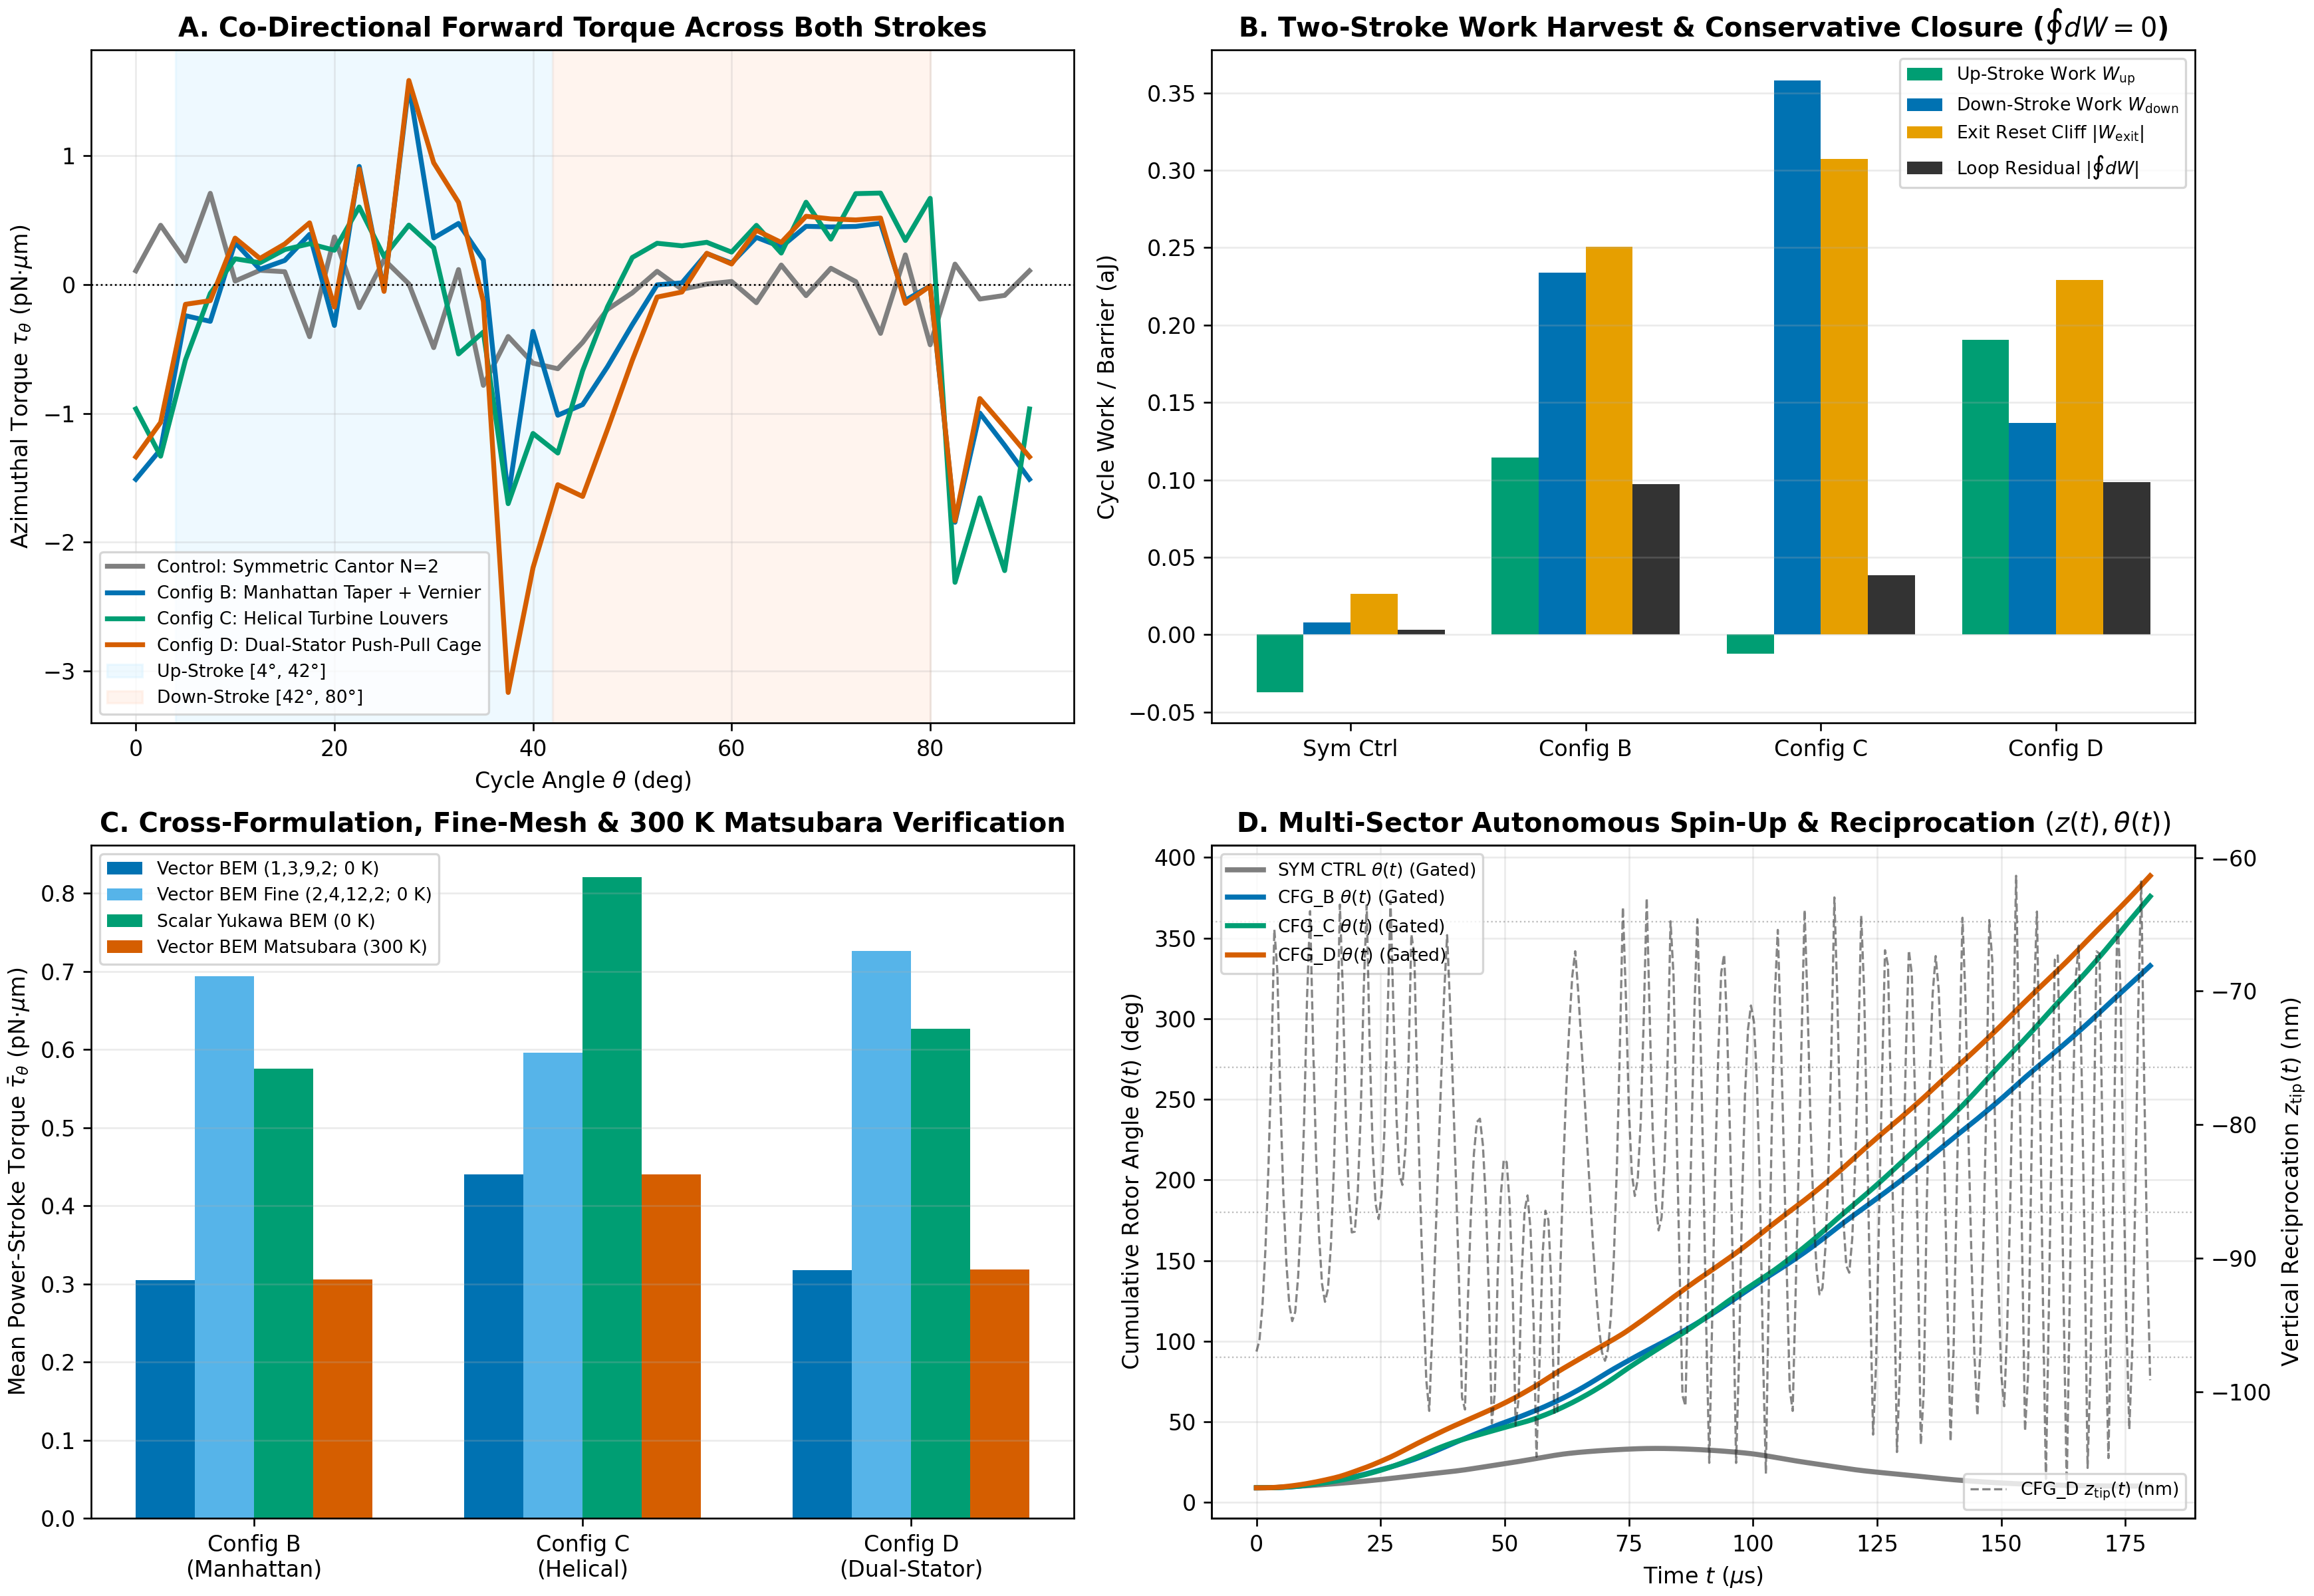
\includegraphics[width=0.96\textwidth]{figures/fig3_engine_strokes_and_dynamics.png}
\caption{Cycle torque profiles, two-stroke work harvest versus conservative exit reset cliff ($|\oint dW| = 0$), cross-formulation and $300\text{ K}$ Matsubara verification, and coupled 2-DOF autonomous spin-up $(z(t),\theta(t))$.}
\label{fig:dynamics}
\end{figure*}

\begin{figure*}[t]
\centering
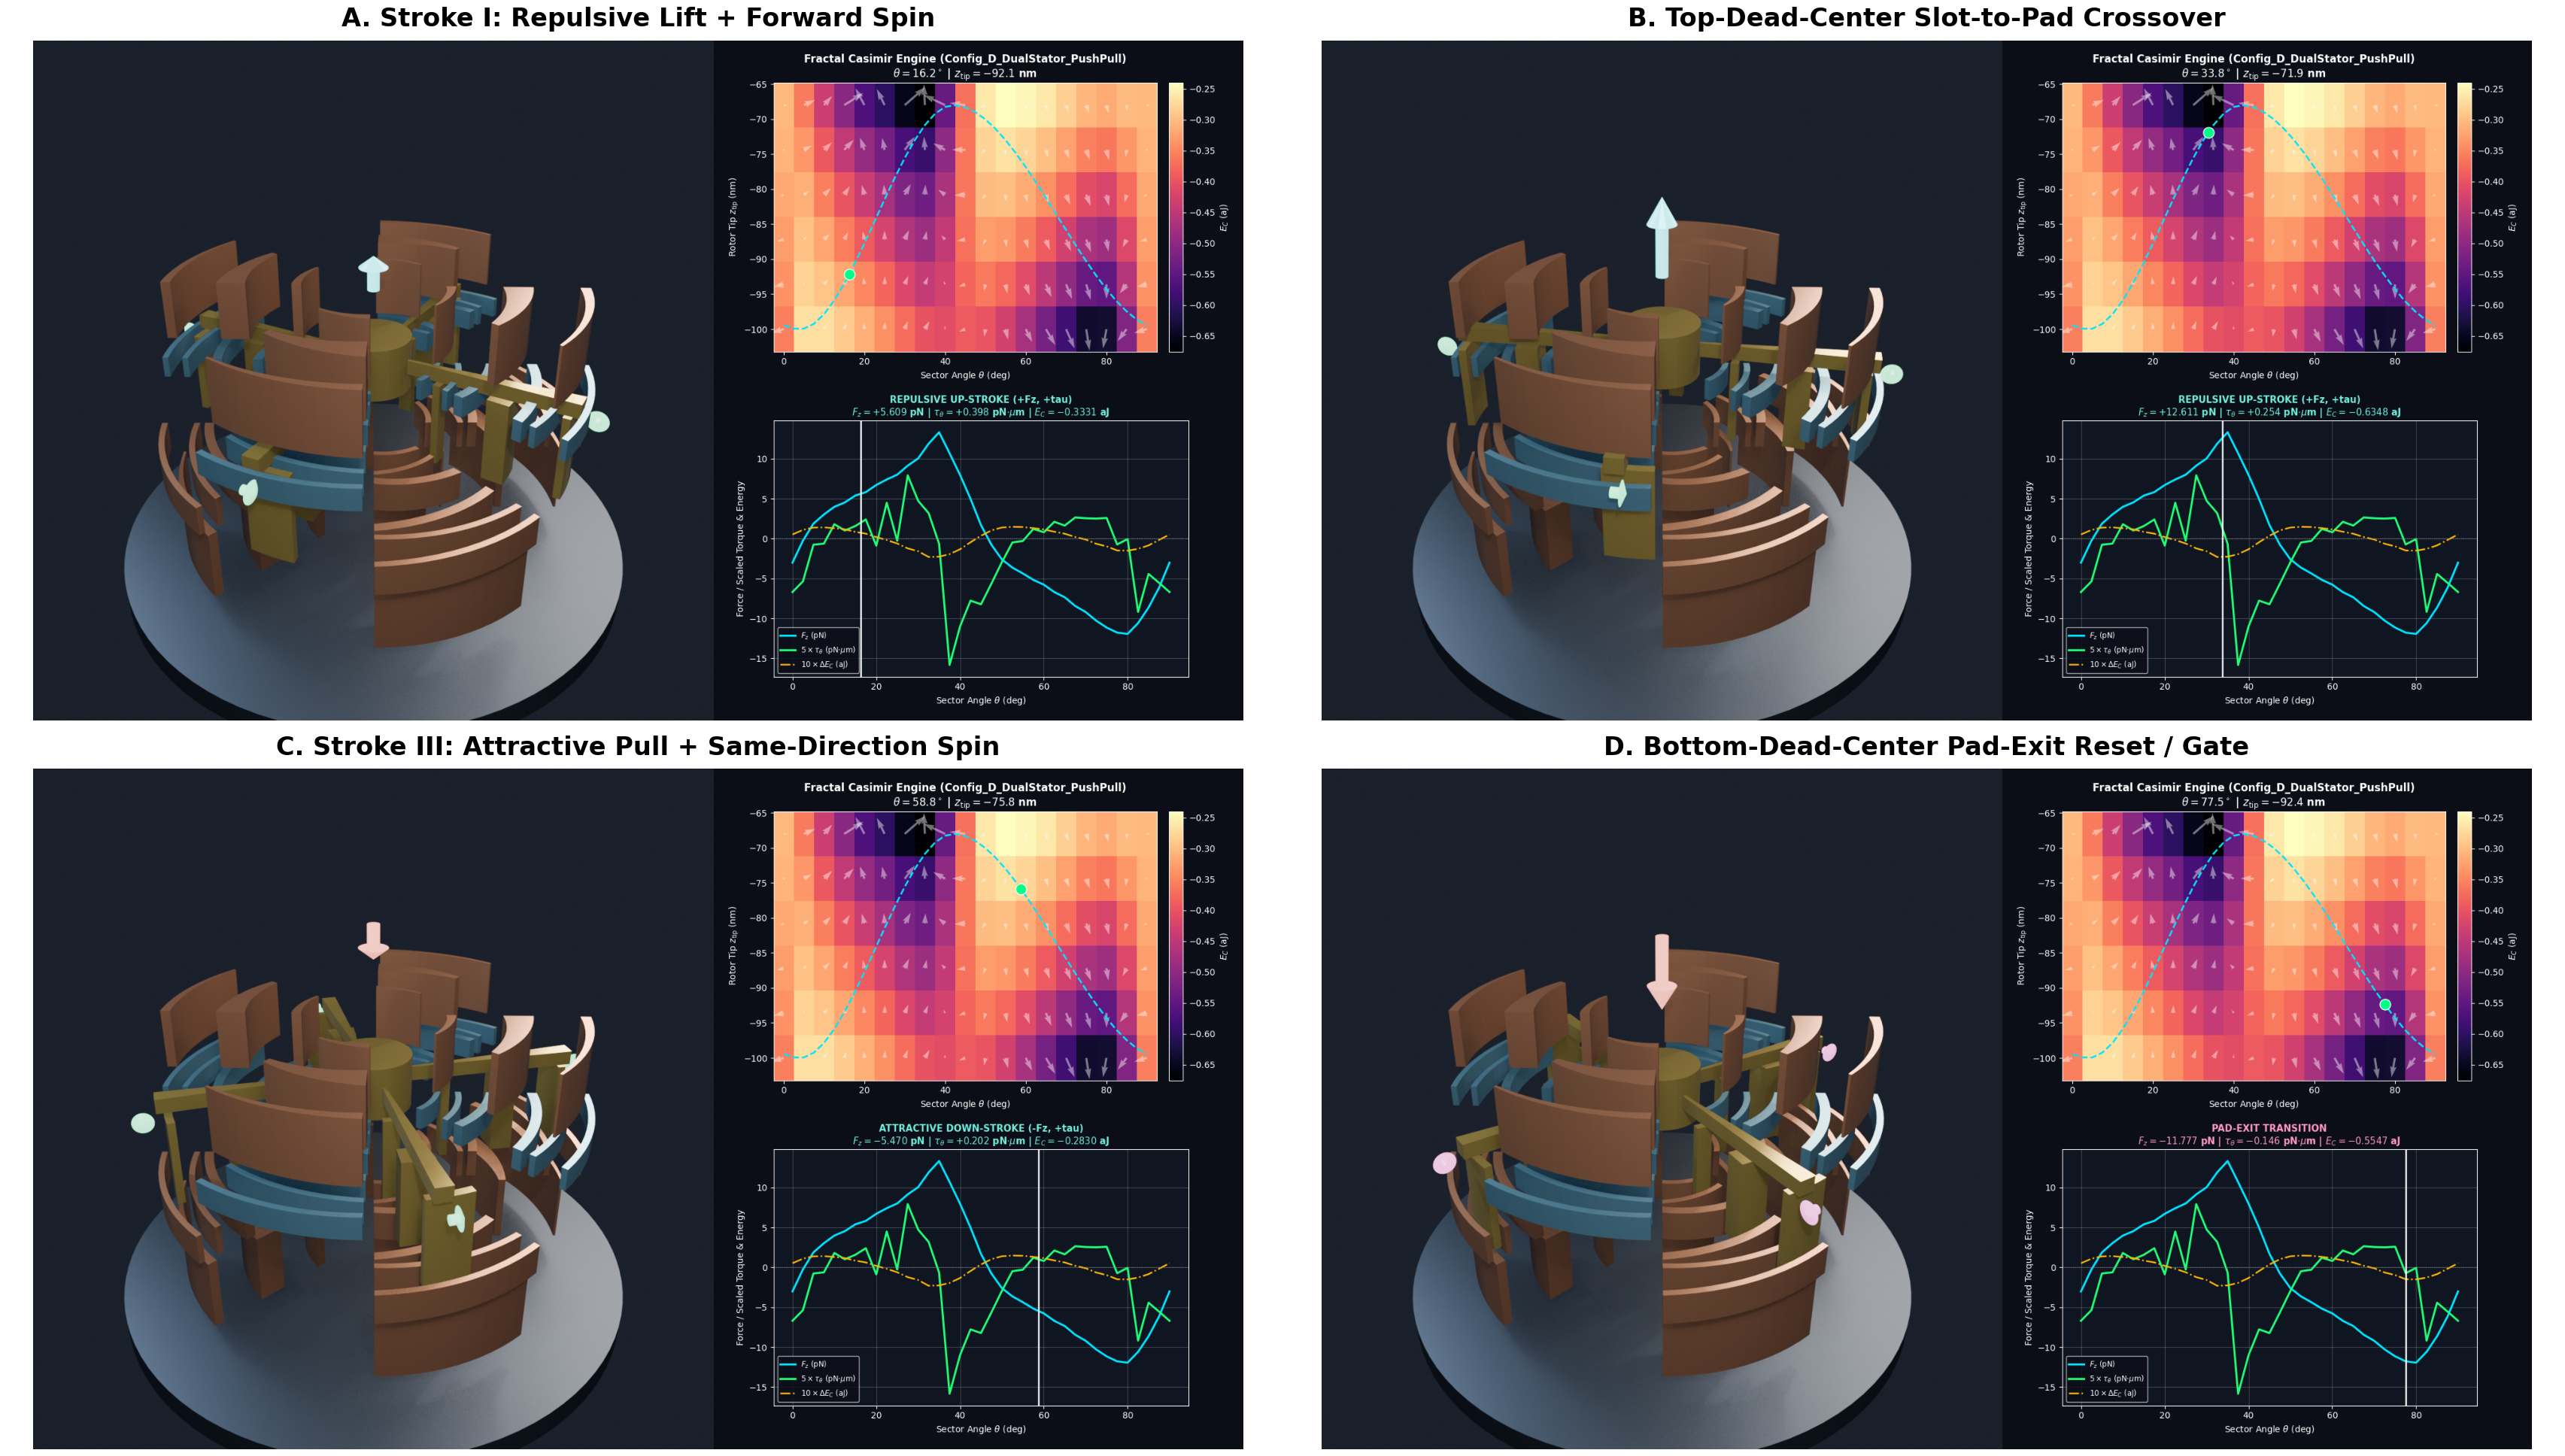
\includegraphics[width=0.96\textwidth]{figures/fig4_engine_blender_keyframes.png}
\caption{Four keyframes from the $\EngineBlenderVideoFrames{}$-frame 3D Blender animation (\texttt{fractal\_casimir\_engine\_cycle.mp4}) of \texttt{Config D}, illustrating dynamic 3D axial force ($F_z$) and tangential torque ($\tau_\theta$) vectors synchronized with live $(z,\theta)$ phase-space telemetry.}
\label{fig:blender}
\end{figure*}

Figures~\ref{fig:landscapes}--\ref{fig:blender} and Table~\ref{tab:engine_benchmarks} summarize the complete cycle mapping:
\begin{enumerate}
    \item \textbf{Simultaneous Repulsive Lift and Forward Torque (Stroke~I)}: While the symmetric control exhibits near-zero symmetry-center torque ($\EngineSymCtrlStrokeOneTauStdPnUm{}\text{ pN}\cdot\mu\text{m}$), all three chiral designs generate positive repulsive lift paired with positive forward torque at $(z_{\rm tip}=-92\text{ nm},\,\theta=22^\circ)$: $(+\EngineCfgBStrokeOneFzStdPn{}\text{ pN},\,+\EngineCfgBStrokeOneTauStdPnUm{}\text{ pN}\cdot\mu\text{m})$ in \texttt{Config B}, $(+\EngineCfgCStrokeOneFzStdPn{}\text{ pN},\,+\EngineCfgCStrokeOneTauStdPnUm{}\text{ pN}\cdot\mu\text{m})$ in \texttt{Config C}, and $(+\EngineCfgDStrokeOneFzStdPn{}\text{ pN},\,+\EngineCfgDStrokeOneTauStdPnUm{}\text{ pN}\cdot\mu\text{m})$ in \texttt{Config D}.
    \item \textbf{Co-Directional Downward Pull and Forward Torque (Stroke~III)}: Over the attractive zone $(z_{\rm tip}=-84\text{ nm},\,\theta=64^\circ)$, axial force flips negative while azimuthal torque remains strictly positive in the \emph{same} forward direction: $(\EngineCfgBStrokeThreeFzStdPn{}\text{ pN},\,+\EngineCfgBStrokeThreeTauStdPnUm{}\text{ pN}\cdot\mu\text{m})$ in \texttt{Config B}, $(\EngineCfgCStrokeThreeFzStdPn{}\text{ pN},\,+\EngineCfgCStrokeThreeTauStdPnUm{}\text{ pN}\cdot\mu\text{m})$ in \texttt{Config C}, and $(\EngineCfgDStrokeThreeFzStdPn{}\text{ pN},\,+\EngineCfgDStrokeThreeTauStdPnUm{}\text{ pN}\cdot\mu\text{m})$ in \texttt{Config D}, preserved across refined Vector BEM, Scalar-Yukawa BEM, and $T=300\text{ K}$ Matsubara dispersion (Table~\ref{tab:engine_benchmarks}).
    \item \textbf{Conservative Loop Closure and Autonomous Engine Spin-Up}: Across the closed $\EngineSectorDeg{}^\circ$ reciprocating trajectory, mechanical work harvested across the contiguous up-stroke ($[4^\circ,42^\circ]$) and down-stroke ($[42^\circ,80^\circ]$) reaches $+\EngineCfgBWorkPowerStrokesAj{}\text{ aJ}$ (\texttt{Config B}), $+\EngineCfgCWorkPowerStrokesAj{}\text{ aJ}$ (\texttt{Config C}), and $+\EngineCfgDWorkPowerStrokesAj{}\text{ aJ}$ (\texttt{Config D}), balanced in static equilibrium by the stator-exit detachment work cliff ($|W_{\rm exit}| = \EngineCfgDBarrierExitAj{}\text{ aJ}$ in \texttt{Config D}, with 36-segment trapezoidal quadrature residual $|\oint dW| = \EngineCfgDLoopResidualAj{}\text{ aJ}$ and exact single-valued loop closure $|E_C(z_0,\EngineSectorDeg{}^\circ)-E_C(z_0,0^\circ)| = 0$). Evaluating the coupled 2-DOF rigid-body dynamics on the $C^1$-conservative periodic bicubic Hermite potential $E_H(z,\theta)$ matching $(E_C,-F_z,-\tau_\theta)$ at every BEM grid node confirms strictly bounded single-sector motion in conservative ballistic release ($\Delta\theta = +\EngineCfgDBallisticNetDeg{}^\circ$ in \texttt{Config D}), whereas suppressing both stator-segment termination cliffs (TDC collar exit and BDC landing-pad exit) via an identical wrap-around unpolarized permittivity gate with zero external torque leaves the symmetric control stationary ($+\EngineSymCtrlReleaseNetDeg{}^\circ$) while unlocking continuous multi-sector rotation reaching $+\EngineCfgBReleaseNetDeg{}^\circ$ (\texttt{Config B}, peak $\EngineCfgBReleasePeakOmegaKrad{}\text{ krad/s}$), $+\EngineCfgCReleaseNetDeg{}^\circ$ (\texttt{Config C}, peak $\EngineCfgCReleasePeakOmegaKrad{}\text{ krad/s}$), and $+\EngineCfgDReleaseNetDeg{}^\circ$ (\texttt{Config D}, peak $\EngineCfgDReleasePeakOmegaKrad{}\text{ krad/s}$) as the rotor reciprocates vertically across its $\EngineStrokeNm{}\text{ nm}$ stroke.
\end{enumerate}

\section{Conclusion}
\label{sec:conclusion}

By breaking azimuthal reflection symmetry oppositely in upper repulsive Cantor slot collars and lower attractive Cantor landing pads, we have demonstrated that vacuum Casimir repulsion and attraction can both drive unidirectional forward torque across a reciprocating axial stroke. Among the three chiral candidates, \texttt{Config B} offers immediate Manhattan EBL manufacturability, \texttt{Config C} provides smooth continuous helical torque transfer, and \texttt{Config D} achieves the highest dual-stroke work density and rotational acceleration.

\bibliographystyle{unsrt}
\bibliography{references}

\end{document}
